%-----------------------------------------------------------------------------%
\chapter{\babDua}
%-----------------------------------------------------------------------------%
This chapter contains the literature reviews which used as the basis of this research. The Software Product Lines, Abstract Behavioral Specification, and related work about feature grouping are explained in this chapter. Additionally, a brief explanation about enterprise software included in this chapter as it will be used as the case study for this research.

%-----------------------------------------------------------------------------%
\section{Software Product Lines}
%-----------------------------------------------------------------------------%
Common software development is focused in developing individual software one at a time to individual users (or market segment). The process starts with analyzing the user's needs, then doing the design, implementation, testing, and last deployment of the software. It could take more efforts and times to build software for individual users. One concept to address this challenge is Software Product Lines. It aims to reduce effort and time of development of each software for individual users in a similar domain \citep{book.apel.FeatureOrientedSoftware}.

The concept of Software Product Lines (SPL) is to build softwares from reusable software components instead of from scratch so that software development can be done more efficiently \citep{book.apel.FeatureOrientedSoftware}. By using the components which already prepared before, the software will be built according to the needs of each user. The softwares produced can be similar in one domain, but they are actually different because they are tailored for the specific needs of users \citep{paper.kastnerApel.FeatureOrientedSoftwareDevelopment}.

There are several promised benefits by using SPL concept \citep{book.apel.FeatureOrientedSoftware,paper.kastnerApel.FeatureOrientedSoftwareDevelopment,book.pohl2005.softwareProductLineEngineering}. First, the software could be produced faster because the development process which uses reusable components. Second, it can reduce the effort and cost because the reusable components have already done before and the users don't need to pay for the cost of design and development software from scratch. Then, it can improve quality because the reusable components can be checked and tested either in isolation or in many softwares. Last, the softwares produced could be tailored for specific needs of users.

%-----------------------------------------------------------------------------%
\subsection{Features}\label{SecFeatures}
%-----------------------------------------------------------------------------%
SPL uses feature-oriented approach in managing variability of the needs or requirements of users. In feature-oriented approach, the variability is represented by using features \citep{paper.kastnerApel.FeatureOrientedSoftwareDevelopment}. A feature is a software property that is used to capture commonalities or variabilities among software \citep{paper.czarnecki2005.mappingFeatureToModels}. For example, for {\it Chat} program, there are features such as {\it Text, Voice, Video Communication}, and so on.

The variability needs to be modeled in order to manage it. One approach to model the variability is using the feature model \citep{book.apel.FeatureOrientedSoftware,paper.kastnerApel.FeatureOrientedSoftwareDevelopment} and represented graphically by using feature diagram \citep{book.apel.FeatureOrientedSoftware}. The feature model will be discussed in section \ref{SecFM} and section \ref{SecFD}.

%-----------------------------------------------------------------------------%
\subsection{Feature Model}\label{SecFM}
%-----------------------------------------------------------------------------%
In SPL, one approach to express variability is by using feature model \citep{book.apel.FeatureOrientedSoftware}. According to \citep{paper.kastnerApel.FeatureOrientedSoftwareDevelopment}, a feature model is a model which describes the set of features and the relationships them. By using feature model, a valid choice of features can be shown \citep{book.apel.FeatureOrientedSoftware}. To represent the feature model in graphical notation, a standard representation is using feature diagram.

%-----------------------------------------------------------------------------%
\subsection{Feature Diagram}\label{SecFD}
%-----------------------------------------------------------------------------%
"A feature diagram is a graphical notation to specify a feature model"  \citep{book.apel.FeatureOrientedSoftware}. A feature diagram is a hierarchical representation like tree representation. In feature diagram, a node consists the feature name denotes a feature. Then, the root representing a concept (e.g., a software system) and its descendant nodes being features. The edges between the node describes their relationships, such as a node connected with empty bullet denotes an optional features and a node connected with filled bullet denotes a mandatory features. If a feature is mandatory, it must be selected whenever the parent feature is selected. Then, multiple a set of child features can be selected only one (alternative) or can be selected more than one (at least 1). The alternative features denoted by empty arch and the 'at least 1' features denoted by filled arch \citep{paper.kastnerApel.FeatureOrientedSoftwareDevelopment}. An example of feature diagram is shown in Figure \ref{fig:ExampleFD}.

\begin{figure}
	\centering
	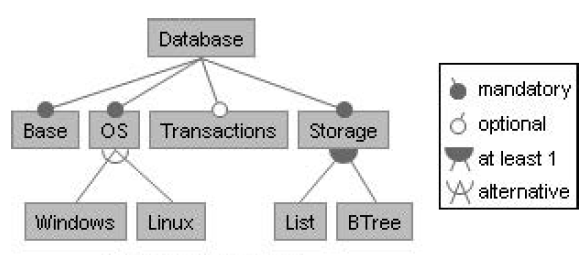
\includegraphics[width=0.6\textwidth]
	{pics/ExampleFD.png}
	\caption{Feature Diagram Example of a Small Database Product Line}
	\label{fig:ExampleFD}
\end{figure}
\vspace{-1cm}
\begin{center}
	{\small Source: \citep{paper.kastnerApel.FeatureOrientedSoftwareDevelopment}}
\end{center}

%-----------------------------------------------------------------------------%
%-----------------------------------------------------------------------------%
%-----------------------------------------------------------------------------%
\section{Abstract Behavioral Specification}
%-----------------------------------------------------------------------------%
Abstract Behavioral Specification (ABS) is a language which developed for high variability and configurable software such as software product lines (SPL) \citep{paper.clarke.variability,paper.hanle.ABStutorial}. As said in \citep{paper.clarke.variability}, "ABS is designed to fill the niche between design-oriented formalisms such as UML and feature description language FDL, on one hand, and implementation-oriented formalisms such as Spec\# and JML, on the other hand". So ABS is a modeling language but it can be executed and generated to other languages such as Java, Maude, or Scala \citep{paper.hanle.ABStutorial}.

ABS was developed by researchers in HATS (Highly Adaptable and Trustworthy Software using Formal Models) project \citep{thesis.niken.deltaRelationalMappingUsingABS} and equipped with ABS tool suite \citep{paper.wong.abstools}. ABS tool suite consists several tools which assist modeling in ABS such as compiler front-end, code generator, ABS plugin, etc. ABS front-end compiler used for code checking and translation code into an internal representation. Then the code generator, use the internal representation and generate it into other languages like Java, Scala, and Maude. To provide editing, visualizing, type checking, and executing, ABS can be integrated with Eclipse IDE which extended by ABS plugin \citep{paper.wong.abstools}.

The architecture of ABS is separated into two groups of layers, namely Core ABS and Full ABS \cite{paper.hanle.ABStutorial}. Core ABS consists several layers which provides modern programming languages like Java or Scala, concurrency, synchronization, standard contracts, and behavioral interface. Above the layers of Core ABS, there are extensions which provide product line engineering, deployment components, and runtime components. These extensions layer called the Full ABS. The architecture of ABS shown in Figure \ref{fig:ArchitectureOfABS}.

\begin{figure}
	\centering
	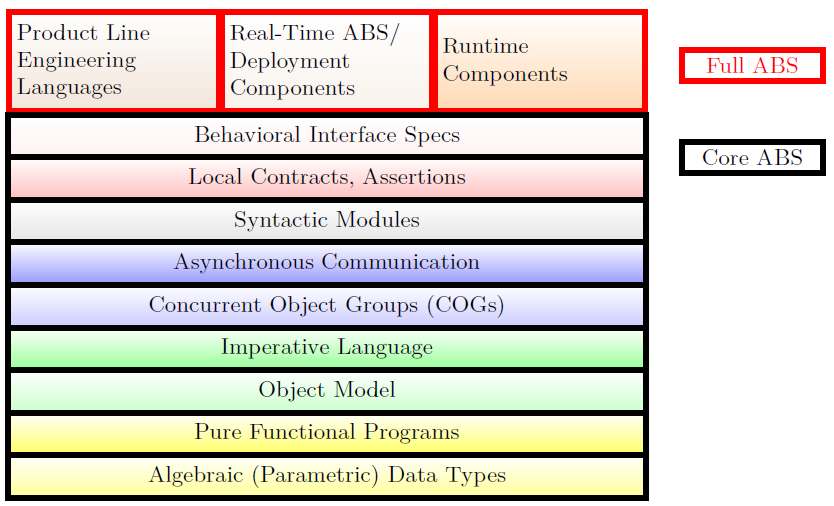
\includegraphics[width=0.8\textwidth]
		{pics/ArchitectureOfABS.png}
	\caption{The Architecture of ABS Language}
	\label{fig:ArchitectureOfABS}
\end{figure}
\vspace{-1cm}
\begin{center}
	{\small Source: \citep{paper.hanle.ABStutorial}}
\end{center}

In section \ref{SPLABS}, product line engineering in ABS is explained more. Then the ABS Compiler, as a part of the ABS tool suite, is explained in section \ref{ABSCompiler}.

%-----------------------------------------------------------------------------%
\subsection{Software Product Line in ABS}\label{SPLABS}
%-----------------------------------------------------------------------------%
SPL is an extension from the Core ABS. There are four special languages to represent product line in ABS \citep{paper.clarke.variability,paper.hanle.ABStutorial}, which are:
\begin{itemize}
	\item Micro Textual Variability Language ($\mu$TVL).
	This language is used to express the variability using feature models. The discussion about feature models in ABS is in section \ref{FeatureModelABS}.
	
	\item Delta Modeling Language (DML).
	This language is used to express the code-level variability of ABS. Delta used to specify transformation of the core ABS code, such as additions, removals, or modifications some methods or attributes. Delta modeling discussed more in section \ref{DeltaModeling}.
	
	\item Product Line Configuration Language (CL).
	This language is used to define the relationships between the feature model and the deltas. Product line configuration discussed more in section \ref{ProductLineConf}.
	
	\item Product Selection Language (PSL).
	This language is used to represent the softwares which can be generated. By define the selected features, a software can be generated. Product selection language discussed more in section \ref{ProductSelection}.
\end{itemize}

The relationship between these languages is shown in Figure \ref{fig:RelationshipFourLanguages}.

\begin{figure}
	\centering
	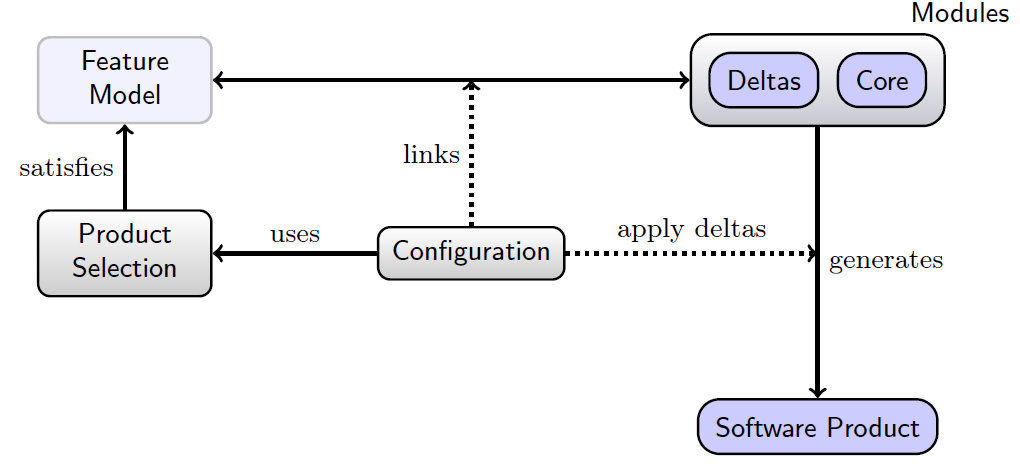
\includegraphics[width=0.7\textwidth]
	{pics/RelationshipFourLanguages.png}
	\caption{Relationship Between the Four Languages}
	\label{fig:RelationshipFourLanguages}
\end{figure}
\vspace{-1cm}
\begin{center}
	{\small Source: \citep{paper.clarke.variability}}
\end{center}


\subsubsection{Feature Models in ABS}\label{FeatureModelABS}
ABS has its feature model. All features will be declared in the feature model.
Johnsen \citep{paper.johnsen2014.deploymentVariabilityinDeltaOriented} gives the definition of feature model in ABS below.

\begin{quote}
	A feature model in ABS is represented textually as a forest of nested features where each tree structures the hierarchical dependencies between related features, and each feature in a tree may have a collection of Boolean or integer attributes. The ABS feature model can also express other cross-tree dependencies, such as mandatory and optional sub-features, and mutually exclusive features.
\end{quote}

The feature modeling language in ABS is using micro textual variability language ($\mu$TVL). $\mu$TVL is an extended subset of textual variability language (TVL). The design of $\mu$TVL is simpler than TVL in order to capture the essential feature modeling requirements \citep{paper.clarke.variability,paper.hanle.ABStutorial}. Beside that, it chosen because $\mu$TVL has formal semantics \citep{thesis.niken.deltaRelationalMappingUsingABS}.

$\mu$TVL has a grammar that shown in Figure \ref{fig:grammarFM}. For each feature, there is an identifier (which is name), an optional group of sub features, optional attributes, and optional constraints \citep{paper.clarke.variability,paper.hanle.ABStutorial}. Based on the grammar, FID denotes a name of a feature and then AID denotes a name of an attribute. Each sub feature has a group cardinality:
\begin{itemize}
	\item {\bf allof}. Indicates that all of the features can be chosen.
	\item {\bf oneof}. Indicates that just one of the features can be chosen (alternative).
	\item $n_{1}$ .. *. Indicates that the number of features can be chosen is from $n_{1}$ to all.
	\item $n_{1}$ .. $n_{2}$. Indicates that the number of features can be chosen is from $n_{1}$ to $n_{2}$.
\end{itemize}

\begin{figure}
	\centering
	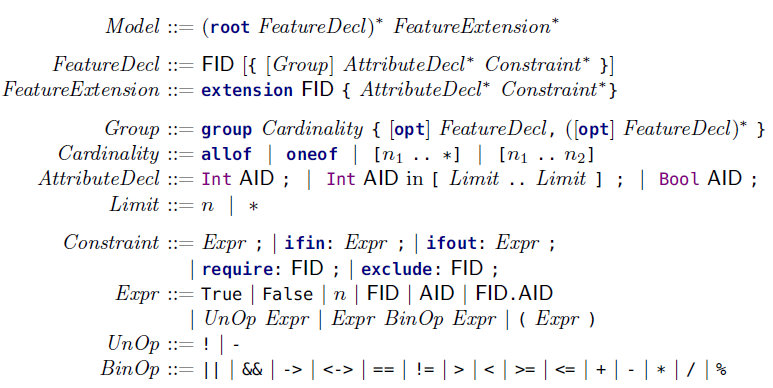
\includegraphics[width=0.9\textwidth]
	{pics/grammarFM.png}
	\caption{Grammar of $\mu$TVL}
	\label{fig:grammarFM}
\end{figure}
\vspace{-1cm}
\begin{center}
	{\small Source: \citep{paper.clarke.variability}}
\end{center}

The {\it AttributeDelc} clause specifies the declaration of attributes of a feature which can be an integer and boolean. An attribute or a feature could have constraints. That constraints is specified by the {\it Constraint} clause. There are several restrictions in the {\it Constraint} clause:
\begin{itemize}
	\item {\bf ifin:} {\it constraint}. Specifies that the {\it constraint} will be applied if the current feature {\bf is} selected.
	\item {\bf ifout:} {\it constraint}.  Specifies that the {\it constraint} will be applied if the current feature {\bf is not} selected.
	\item {\bf require:} FID. Specifies that the current feature needs the presence of other feature (which specifies with FID).
	\item {\bf exclude:} FID. Specifies that the current feature cannot be chosen if the other feature (which specifies with FID) is chosen, and vice versa.
\end{itemize}

An example of feature model in ABS is shown in Listing \ref{codeFMAccount}. The example shows the code of feature model for {\it Account} features. There are six features, group of sub features, constraints and attributes for the features. It also shows the features that optional (denotes with {\bf opt}) and mandatory (denotes without {\bf opt}).

\lstinputlisting[
	label={codeFMAccount},
	caption={Exampe Account Feature Model in ABS \citep{paper.hanle.ABStutorial}},
	firstline=1,
	style=ABS]{src/AccountFeatureModel.abs}

\subsubsection{Delta Modeling}\label{DeltaModeling}
Delta modeling uses the delta-oriented programming approach. Delta-oriented programming is an approach in SPL as an alternatives to feature-oriented programming approach \citep{paper.clarke.variability}. In delta-oriented programming, the aim is to provide a technique in generating software which modular and flexible in SPL \citep{paper.clarke.variability,paper.johnsen2014.deploymentVariabilityinDeltaOriented,paper.schulze2013.refactoringDeltaOrientedSPL}. Delta-oriented programming uses \textit{delta modules (deltas)} which the modules are associated with program modifications (add, remove, or modify code) \citep{paper.clarke.variability}. It's different from feature-oriented programming  which uses feature modules \citep{paper.kastnerApel.FeatureOrientedSoftwareDevelopment} that associated with each features \citep{paper.clarke.variability,paper.schulze2013.refactoringDeltaOrientedSPL}.

The implication of not associating delta module directly with features, it can obtain the flexibility, better code reuse, and get the ability to resolve conflicts when applying other delta modules \citep{paper.clarke.variability}. Other benefit of deltas is the abilities of delta module. A delta module can add, remove, and modify code. 

\begin{figure}
	\centering
	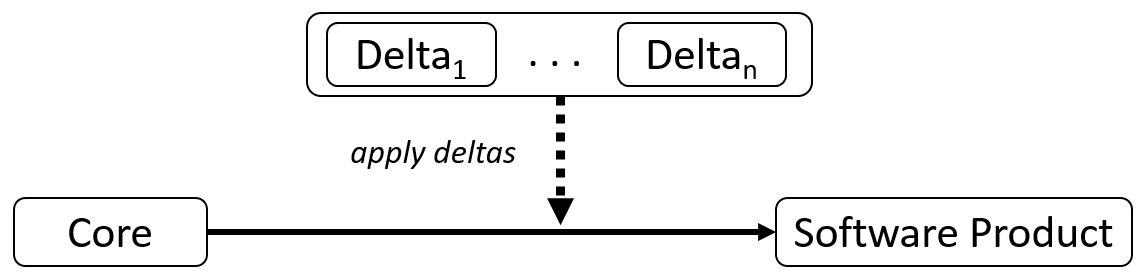
\includegraphics[width=0.9\textwidth]
	{pics/applicationOfDelta2.png}
	\caption{The Application of Delta Modules}
	\label{fig:applicationOfDelta}
\end{figure}
\vspace{-1cm}
\begin{center}
	{\small Source: \citep{paper.hanle.ABStutorial}}
\end{center}

There are two divisions of implementation of SPL in delta-oriented programming \citep{paper.clarke.variability,paper.johnsen2014.deploymentVariabilityinDeltaOriented}. They are core modules and delta modules. The core modules consist classes which implement a complete software for the SPL. Then, to obtain a new variant of software, the delta modules are used to describe how to modify the core modules. The application of delta modules to get a new software variant is shown in Figure \ref{fig:applicationOfDelta}.

\subsubsection{Product Line Configuration}\label{ProductLineConf}
Product line configuration (CL) uses to link the features in feature model with the delta modules so it can provide a complete specification for the product line \citep{paper.clarke.variability,paper.hanle.ABStutorial,paper.johnsen2014.deploymentVariabilityinDeltaOriented}. The declarations of which deltas applied to which features are written in here. Thus, it can make the process of analyzing the whole product lines more efficient \citep{paper.hanle.ABStutorial}.

Product line configuration consists set of features and set of delta modules. The connection between feature model, delta module, and the product line configuration is shown in Figure \ref{fig:connectionFmodDmodCL}. There are three configurations that could be specified in CL \citep{paper.hanle.ABStutorial,paper.johnsen2014.deploymentVariabilityinDeltaOriented}:
\begin{itemize}
	\item \textit{application condition} \\
	The \textit{application condition}, which denoted by \code[style=abs]{when} clause, associates the delta modules with the features. It describes that if the feature is selected, then use this delta(s) to implement the product line.
	
	\item \textit{parameters} \\
	The \textit{parameters} are derived from the feature attribute values which will be passed to the delta module.
	
	\item \textit{order of delta application} \\
	The \textit{order of delta application}, which denoted by \code[style=abs]{after} clause, is used to ensure the application of deltas is well-defined and resolve conflicts which could be occurred.
\end{itemize}

\begin{figure}
	\centering
	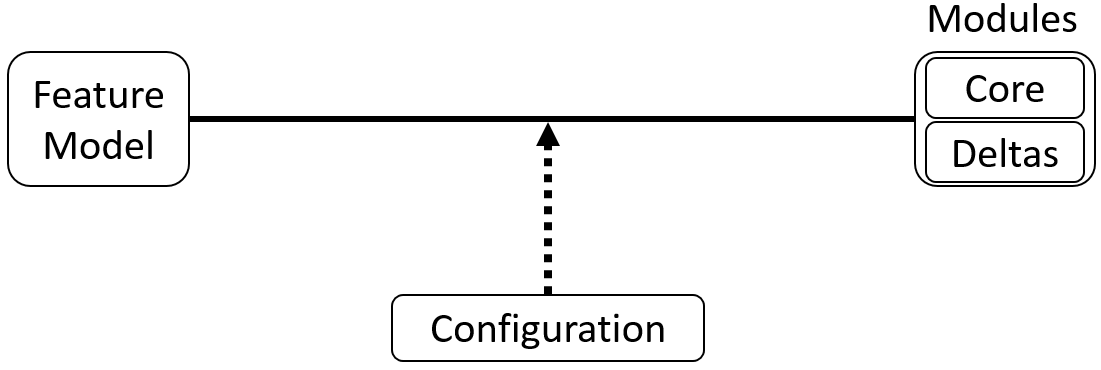
\includegraphics[width=0.7\textwidth]
	{pics/connectionFmodDmodCL2.png}
	\caption{The Connection Between Feature Model, Deltas, and CL}
	\label{fig:connectionFmodDmodCL}
\end{figure}
\vspace{-1cm}
\begin{center}
	{\small Source: \citep{paper.hanle.ABStutorial}}
\end{center}

An example of product line configuration shown in Listing \ref{codeAccountPL}. It is a configuration for the {\it Accounts} product line (which the features are shown in section \ref{FeatureModelABS}).

\lstinputlisting[
	label={codeAccountPL},
	caption={Account Product Line Configuration \citep{paper.hanle.ABStutorial}},
	firstline=1,
	style=ABS]{src/AccountPL.abs}


\subsubsection{Product Selection Language}\label{ProductSelection}
To specify the products (softwares) that could be generated, ABS uses the product selection language (PSL). Product selection language describes the features which will be included in the product and gives values to the attributes if needed \citep{paper.clarke.variability,paper.hanle.ABStutorial,paper.johnsen2014.deploymentVariabilityinDeltaOriented}. The syntax of PSL is pretty simple. To specify a product, the elements needed are the product name, the features used in that product, and values of attributes, if needed, to the features.

The example of product selection language is shown in Listing \ref{codeAccountProducts}. There are examples of products of {\it Accounts} product line. For example, \textit{CheckingAccount} product is built from \textit{Type} feature and \textit{Check} feature.

\lstinputlisting[
	label={codeAccountProducts},
	caption={PSL of Account Product Line \citep{paper.hanle.ABStutorial}},
	firstline=1,
	style=ABS]{src/AccountProducts.abs}


%-----------------------------------------------------------------------------%
\subsection{ABS Compiler}\label{ABSCompiler}
%-----------------------------------------------------------------------------%
ABS has a tool suite that used as a platform for developing and analyzing the ABS code \citep{paper.wong.abstools}. In ABS tool suite, there are two tools that used to be a compiler. They are compiler front-end and compiler back-end. The process to compile the ABS code and generate it to be a other language is shown in Figure \ref{fig:ABScompilerFlow}. ABS compiler front-end is used to translate the ABS code into an internal representation, then the ABS compiler back-end will use the internal representation to generate other languages.

\begin{figure}
	\centering
	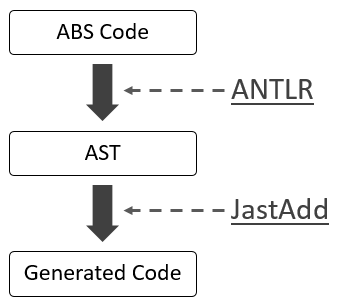
\includegraphics[width=0.5\textwidth]
	{pics/ABScompilerFlow.png}
	\caption{ABS Compiler Process Flow}
	\label{fig:ABScompilerFlow}
\end{figure}

In section \ref{ABSFrontEnd}, ABS compiler front-end is explained more. Then, the explanation of ABS compiler back-end is in section \ref{ABSBackEnd}.  

%-----------------------------------------------------------------------------%
\subsubsection{ABS Compiler Front-End}\label{ABSFrontEnd}
%-----------------------------------------------------------------------------%
ABS compiler front-end is used to translate the ABS code into an internal representation \citep{paper.wong.abstools}. The internal representation later will be used to check the ABS code for syntax and semantic errors. The compiler front-end takes ABS codes, such as core, feature model, delta modules, configuration, and product selection as inputs and translates them into the internal representation. From the internal representation of feature model, a valid combination of features can be found and used to validate the product selections.

The internal representation is called the Abstract Syntax Tree (AST) \citep{thesis.niken.deltaRelationalMappingUsingABS,paper.wong.abstools}. AST is a representation of the language constructions and formed as a tree \citep{paper.hedin.jastadd}. To translate ABS code into AST, the ABS compiler front-end uses a tool called ANTLR. ANTLR is a parser generator which can be used to read, process, execute, or translate structured text or binary files \citep{web.ANTLR.aboutANTRLParser}. ANTLR also can build the AST by providing grammar annotations. The grammar annotations used to indicate what tokens are treated as subtree roots, leaves, or to be ignored with respect to tree construction. To construct a tree with special structure, the ANTLR must be provided with the tree definitions \citep{web.ANTLR.ANTRLTreeConstruction}. In ABS, it's located in the abstract grammar which specified in \code{.ast} file.

The abstract grammar is defined in an \code{.ast} file called \code{ABS.ast}. A partial representation of ABS class hierarchy defined in \code{ABS.ast} is shown in Figure \ref{fig:ABSastHierarchy}.

\begin{figure}
	\centering
	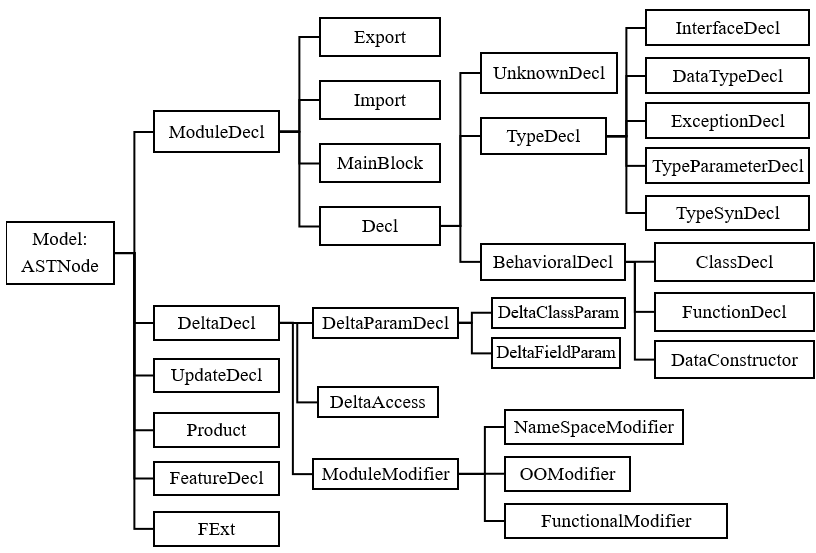
\includegraphics[width=0.8\textwidth]
	{pics/ABSastHierarchy.png}
	\caption{ABS.ast Hierarchy Represented in Diagram}
	\label{fig:ABSastHierarchy}
\end{figure}

%-----------------------------------------------------------------------------%
\subsubsection{ABS Compiler Back-End}\label{ABSBackEnd}
%-----------------------------------------------------------------------------%
The ABS compiler front-end has translated the ABS code into AST, then ABS compiler back-end uses the AST as an input to generate it into other languages. It can generate code to either executable programs in implementation languages, such as Java or Scala, or rewriting systems for simulation and analysis, such as Maude \citep{paper.wong.abstools}. To generate the AST to other languages, ABS uses JastAdd\footnote{http://jastadd.org/web/documentation/concept-overview.php} as the tool.

JastAdd is a meta-compilation system which designed to support extensible implementation of compilers and related tools like analyzers or transformation tools \citep{web.JastAdd.JastAddOverview}. By using JastAdd, the compiler can be extended by adding module that contain new abstract syntax and computations on the AST. The abstract syntax is modeled as a class hierarchy. It's modeled from the corresponding code which generated. 

JastAdd supports a capability for implementing behavior in the form of attributes \citep{web.JastAdd.JastAddOverview}. Attributes are attached to the AST nodes in AST and the values could be integers, composite values like set, or reference values which are stated using equations. Moreover, the values could point to other nodes in AST or access other attributes \citep{thesis.niken.deltaRelationalMappingUsingABS}.

The classes in the hierarchy called AST classes because they model nodes in the AST \citep{web.JastAdd.JastAddOverview}. There are method API formed to the classes which correspond to each attributes. By using the API, a programmer can get the correct value of the attribute according to the equation \citep{thesis.niken.deltaRelationalMappingUsingABS}.

ABS compiler back-end uses the \textit{aspects} of JastAdd to do the code generation. According to \citep{web.JastAdd.JastAddReferenceManual}, JastAdd will read the aspects files and weaves the aspect declarations into the appropriate AST classes. By adding a \code{.jadd} file, the AST classes could be added some ordinary fields and methods \citep{web.JastAdd.JastAddReferenceManual}. Therefore, a behavior could be added to the AST classes such as pretty printing behavior.


%-----------------------------------------------------------------------------%
%-----------------------------------------------------------------------------%
%-----------------------------------------------------------------------------%
\section{Feature Grouping and Related Works}
%-----------------------------------------------------------------------------%
In ABS, a set of features is defined in feature model. Then, the selection of features that will be included in a software is done by writing the features using product selection language (section \ref{ProductSelection}). The feature model can consist a feature tree in implementation level. For example, from Figure \ref{fig:FD1} which shown the example of Home Integrated System feature diagram, a \textit{Heat} feature is a child of \textit{Detector} feature which a child of \textit{Fire} feature. The deep level could be vary based on the feature model.

The feature model also can be very large if the number of features available is increasing, such as Linux kernel with more than 10.000 features \citep{book.apel.FeatureOrientedSoftware}. The selection of features could be more difficult to do. Even more for users to choose the features they want. To address this problem, the features in the feature model can be grouped.

Previous researchers have done researches about how to group the features. Two of those are by using the feature binding unit (FBU) \citep{paper.lee.featurebinding,paper.lee.featuremanagement} and views \citep{paper.hubaux2013.supportingMultiplePerspective}.

%-----------------------------------------------------------------------------%
\subsection{Feature Binding Unit, Lee et al.}
%-----------------------------------------------------------------------------%
Lee et al \citep{paper.lee.featuremanagement} define the feature binding unit (FBU) as: "A set of features that are related to each other by the relationships in a feature model". Feature binding consists a set of features that run a common service an must exist together to perform a the correct service \citep{paper.lee.featurebinding,paper.lee.featuremanagement}. As said by Lee \citep{paper.lee.featuremanagement} that the grouping can reduce the complexity in managing the variations, thus it can reduce the complexity for users to choose the common services they want (even if the product selection language still use features to specify a software).

The examples of feature binding units are shown in Figure \ref{fig:FeatureModelFBU}. The FBU is a set of features denoted by blue-dotted-line circle. For example, there are several basic features, such as {\it Security Basics, Intrusion Basics, Fire Basics, Flood Basics,} and {\it Alarm Basics}. Then there are features grouped to be additional features, such as {\it Additional Fire Services, Voice Communication, Pumping Tool,} and {\it Internet Data Message}. The features are grouped by the common services they provided and the relationship they had in the feature model.

\begin{figure}
	\centering
	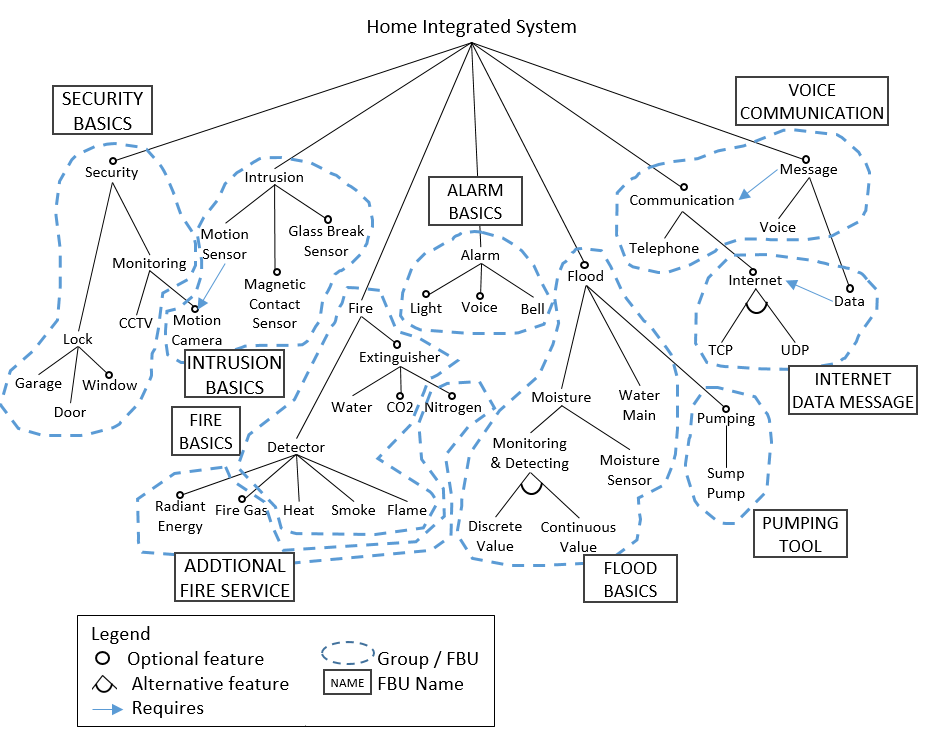
\includegraphics[width=0.8\textwidth]
	{pics/hisfd4group3a.png}
	\caption{Home Integration System Feature Diagram with Grouping}
	\label{fig:FeatureModelFBU}
\end{figure}
\vspace{-1cm}
\begin{center}
	{\small Source: \citep{paper.lee.featurebinding} (with additional changes)}
\end{center}

%-----------------------------------------------------------------------------%
\subsection{Views, Hubaux et al.}
%-----------------------------------------------------------------------------%
Hubaux et al \citep{paper.hubaux2013.supportingMultiplePerspective} said that there are two challenges that failed to address by feature selection process using the original feature model. Those are (1) configuring the feature selection environment according to the users' profile (e.g knowledge, role, preferences, etc) and (2) managing the complexity from the size of the feature diagram.

View is one to address those challenges. Hubaux et al \citep{paper.hubaux2013.supportingMultiplePerspective} define view as: "a simplified representation of a feature diagram that has been tailored to the stakeholders (users) profile or generalized to a particular combination of features". Using view, it facilitate the users to focus only on those parts that are relevant to them. Thus, it could reduce the complexity of choosing the features. 

There are three issues that Hubaux et al focus on. Those are as follow.
\begin{itemize}
	\item View Specification \\
	There are two ways to specify views. First, by enumerating the features that appear for each views. It can be done by tagging each feature with the names of the views they belong to. Second, by using a language that takes advantage of the feature diagram tree structure. They using XPath as the language that designed to navigate in tree-structures.
	
	\item View Coverage \\
	It is important to guarantee that a decision for each feature in feature diagram has been made (selected or not). One way is to fulfill the sufficient coverage condition. Sufficient coverage condition means that all features should appear in at least one view, hence no feature can be left undecided.
	
	\item View Visualization \\
	The views need to be made concrete by using visualization. Hubaux et al define the goal of a visualization are:
	\begin{itemize}
		\item showing only features that belong to a view, and 
		\item including features that are not in the view but that provide context and thereby allow the user to make informed decisions.
	\end{itemize}
\end{itemize}

%-----------------------------------------------------------------------------%
\subsection{Comparison}
%-----------------------------------------------------------------------------%
Previous researchers have attempted to manage the complexity of features selection by grouping the features. Lee et al introduce the feature binding unit (FBU) which each of it consists features that belong to the same service provided. Then Hubaux et al introduce view as a set of features that has been tailored to users profile. Both of them trying to group the features in different ways, but there is no grouping mechanism based on the features domains (e.g. basic or special features for a module), the target of the users (e.g. small or large companies), and so on. Lee et al discuss how to group the features only by their common service. Then Hubaux et al discuss how to group the features in technical terms by tagging each feature with the names of the views (groups) they belong to.


\section{Enterprise Management Software}
As this research uses a part (module) of an enterprise management software, also known as enterprise software or enterprise application software, here is an brief explanation about enterprise software. 

Enterprise software is a software which allows companies to integrate business processes by sharing information across business functions and employee hierarchies \citep{book.olson2010.enterpriseIS}. It can replace multiple independent systems which process data to support particular business functions or processes. A lot of data used in an enterprise software. Fowler in \citep{book.fowler2002.patternsEnterpriseApp} said that an enterprise softwares are about 1) the display, manipulation, and storage of large amounts of data and 2) the support or automation of business processes with that data.

There are several types of enterprise software. Enterprise Resource Planning (ERP), Customer Relationship Management (CRM), and Supply Chain Management (SCM) are examples of enterprise softwares \citep{web.erp.typeEnterpriseSystem}. They support companies to do some business processes more efficiently. For example, an ERP software used to integrate some business processes, such as sales, purchasing, finance, human resources, and inventory management, so it can communicate and share data among departments in a company. In a common way, each function of an enterprise software is called module. So that the function to support sales process is called sales module. Modules in an enterprise software can be different based on the types of the enterprise software.

In conclusion, enterprise softwares are intended to solve an enterprise-wide problem. It aims to improve the enterprise's productivity and efficiency by providing business support functionality. Then, several types of enterprise software are intended to help companies to run their business processes based on the type of the business process.